\chapter{Εισαγωγή}


Στόχος της εργασίας αυτής είναι η ενεργητική ενθάρρυνση συνέχισης του διαλόγου με τον χρήστη ενός διαλογικού συστήματος,
ονόματι Θεανώ \cite{ventoura-etal-2021-theano}, με χρήση ενισχυτικής μάθησης.
Τα θέματα τα οποία κατανοεί η Θεανώ προέρχονται από μια τράπεζα θεμάτων συζήτησης σχετικά με τον \en{Covid-19}
και στοχεύουμε να προτείνονται με τρόπο, ώστε το ενδιαφέρον του χρήστη να διατηρηθεί, χωρίς να κάνει την Θεανώ να φαίνεται παρεμβατική.
Πρακτικά, η εργασία αυτή ασχολείται με την ανάπτυξη ενός συστήματος το οποίο συνδέει τρία βασικά στοιχεία:
τις συστάσεις, τα διαλογικά συστήματα και την ενισχυτική μάθηση. Κάθε ένα από αυτά τα στοιχεία θα αναλυθεί σε βάθος στα επόμενα κεφάλαια.
Σε αυτή την ενότητα θα γίνει μια εισαγωγή στα κίνητρα, τις βασικές ιδέες που χρησιμοποιήθηκαν στην εργασία,
καθώς και τα κύρια χαρακτηριστικά των συστημάτων αυτών, καθώς και των προϋπάρχουσων υποδομών.


\section{Κίνητρα}

Οι διαλογικοί πράκτορες (\en{bots}) δημιουργήθηκαν με σκοπό να μειώσουν τον ανθρώπινο κόπο.
Το όραμα είναι, εκεί που σήμερα υπάρχει ένας άνθρωπος-πράκτορας πάντα διαθέσιμος να εξυπηρετήσει τα ερωτήματα των πελατών/ενδιαφερομένων,
να υπάρχουν αυτόματα διαλογικά συστήματα που να τους εξυπηρετούν με παρόμοια ποιότητα υπηρεσιών.

Η έρευνα στα διαλογικά συστήματα ξεκίνησε από τις αρχές του 1970 με ένα σύστημα βασισμένο σε κανόνες που ονομαζόταν \en{ELIZA}\cite{eliza}
και έχει φτάσει στο απόγειο της πλέον, με την δημιουργία συστημάτων σαν το \en{ChatGPT} και το \en{Mistral}, διαλογικών συστημάτων γενικού σκοπού,
βασισμένα στην αρχιτεκτονική των μετασχηματιστών (\en{transformers}).
Για παράδειγμα, το μοντέλο \en{GPT-3}, το οποίο χρησιμοποιείται στην δωρεάν έκδοση του \en{ChatGPT} έχει 175 δισεκατομμύρια παραμέτρους\cite{brown2020language},
ενώ το \en{GPT-4}, το οποίο παρέχεται στην επί-πληρωμή έκδοση, υπολογίζεται ότι έχει 1.76 τρισεκατομμύρια παραμέτρους. Παρόλα αυτά, η διατήρηση του ενδιαφέροντος
του χρήστη κατά την διάρκεια του διαλόγου και η ενεργητική προσπάθεια για την συνέχιση του, είναι ένα πρόβλημα που πρόσφατα άρχισε να μελετάται, και συνεπώς δεν έχει
λυθεί επαρκώς - ειδικά όταν ο πράκτορας έχει συγκεκριμένο πεδίο γνώσεων.

Επιπλέον, το πρόβλημα της διαχείρισης διαλόγων με πολλούς γύρους είναι ένα πρόβλημα που επίσης είναι σχετικά νέο στην βιβλιογραφία\cite{yi2024surveyrecentadvancesllmbased}\cite{ni2022recentadvancesdeeplearning}.
Μια παρόμοια κατηγορία διαλογικών συστημάτων, είναι τα προορατικά (\en{proactive}) διαλογικά συστήματα, τα οποία έχουν ως σκοπό να κατευθύνουν την συζήτηση με τον χρήστη
προς κάποιο συγκεκριμένο στόχο/σκοπό. Η έρευνα για αυτά τα συστήματα είναι πολύ πρόσφατη και συνήθως, όταν αναφέρεται σε συστήματα με συγκεκριμένο σκοπό, εστιάζει στο
να εξάγει περισσότερες πληροφορίες σχετικά με το αίτημα του χρήστη ή να προσφέρει περισσότερες πληροφορίες με βάση τη ήδη υπάρχοντα ερωτήματα του χρήστη\cite{Deng2023ASO}.

Σκοπός της διπλωματικής εργασίας, λοιπόν, είναι η δημιουργία ενός συστήματος σύστασης ενδιαφερόντων θεμάτων για τον χρήστη, τα οποία προέρχονται μέσα από μια προκαθορισμένη τράπεζα θεμάτων.
Ο παραπάνω στόχος θα επιτευχθεί για το διαλογικού συστήματος Θεανώ, το οποίο δημιουργήθηκε στο ΕΚ Αθηνά.
Η Θεανώ είναι ένα διαλογικό σύστημα, το οποίο μπορεί να απαντήσει καίρια ερωτήματα σχετικά με τον \en{Covid-19}.
Ως ενδιαφέροντα θέματα ορίζονται τα θέματα τα οποία θα επιτύχουν να διατηρήσουν την αλληλεπίδραση με τον χρήστη για μεγαλύτερη διάρκεια (ή πιο φορμαλιστικά για περισσότερους γύρους διαλόγου).
Έτσι, για παράδειγμα, ένας χρήστης θα ρωτήσει κάποια ερώτηση, και αφού το σύστημα απαντήσει,
θα του προτείνει και ένα θέμα περαιτέρω συζήτησης, με βάση τα θέματα τα οποία έχει στην τράπεζα θεμάτων.

Όπως είναι προφανές, κάθε χρήστης έχει διαφορετικό ιστορικό, διαφορετικά ενδιαφέροντα και διαφορετικές πληροφορίες που θέλει να μάθει.
Πολλά από αυτά τα χαρακτηριστικά του χρήστη δεν είναι ποτέ διαθέσιμα σε εμάς, ενώ άλλα γίνονται εμφανή κατά την διάρκεια του διαλόγου.
Έτσι, το σύστημα θα πρέπει να μπορεί να κάνει δύο πράγματα. Το πρώτο είναι να μπορεί να κατανοήσει τα θέματα συζήτησης που σχετίζονται νοηματικά και
είναι πιθανό ότι αν ο χρήστης ρωτήσει για το ένα, να ενδιαφέρεται και για το άλλο. Το δεύτερο είναι να μπορεί να κατανοήσει τα ενδιαφέροντα του χρήστη με βάση τις
ερωτήσεις που κάνει και τα θέματα που επιθυμεί να μάθει ή όχι. Καθώς οι χρήστες δεν είναι γνωστοί από πριν, και τα ενδιαφέροντα θέματα συζήτησης μπορεί να
αλλάζουν ανά περίοδο, η χρήση κλασικής επιβλεπόμενης μάθησης δεν είναι εφικτή. Αυτό συμβαίνει γιατί στην επιβλεπόμενη μάθηση χρειάζονται γνωστά
δείγματα και σωστές απαντήσεις σε αυτά δείγματα, οι οποίες δεν υπάρχουν σε αυτή την περίπτωση, καθώς δεν υπάρχει μια ξεκάθαρη ανάγκη για τους χρήστες.
Αντίθετα χρειάζεται μια πιο δυναμική προσαρμογή, η οποία επιτυγχάνεται μέσω την σύγχρονης μάθησης \en{(online learning)} και της ενισχυτικής μάθησης
\en{(reinforcement learning)}.

\section{Η Θεανώ}

\begin{figure}
    \centering
    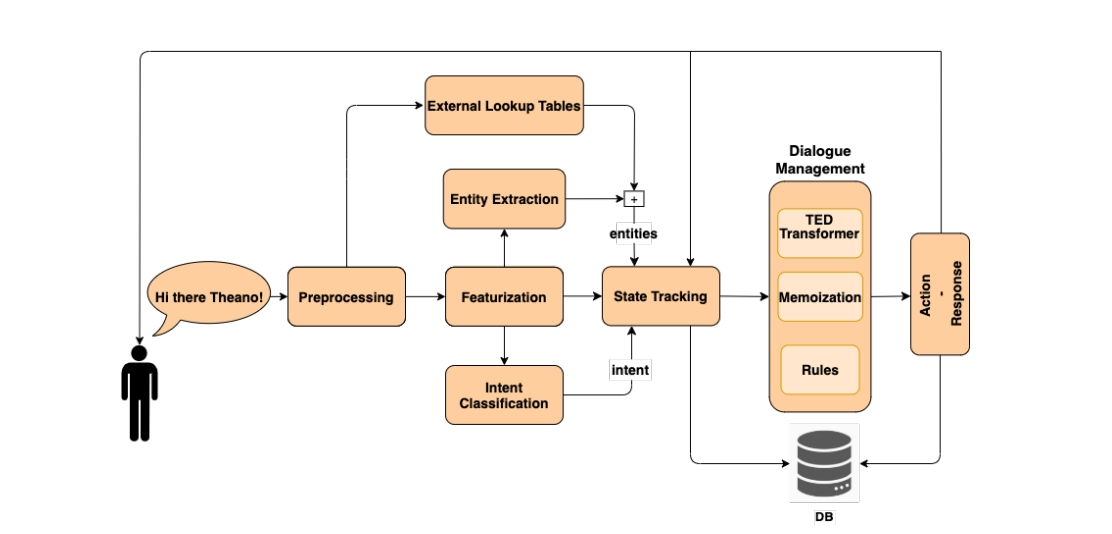
\includegraphics[width=\textwidth]{body_matter/introduction/images/theano-architecture.jpeg}
    \caption{Η αρχιτεκτονική της Θεανώς}
    \label{fig:theano_architecture}
\end{figure}

Η Θεανώ είναι ένας διαλογικός πράκτορας που έχει σκοπό την ενημέρωση σχετικά με τον \en{Covid-19}\cite{ventoura-etal-2021-theano}.
Έχει χτιστεί με βάση την εργαλειοθήκη \en{Rasa}, η οποία παρέχει ένα ολοκληρωμένο διαλογικό σύστημα από άκρη σε άκρη.
Συγκεκριμένα, όπως φαίνεται και στο Σχήμα \ref{fig:theano_architecture}, το \en{Rasa} παρέχει σύστημα κατανόησης της φυσικής γλώσσας,
ένα σύστημα αναγνώρισης των προθέσεων του συνομιλητή (\en{intent classification}) και επιλογής της κατάλληλης απάντησης με βάση αυτό (\en{state tracking}).
Τέλος, έχει και ένα σύστημα παραγωγής φυσικής γλώσσας για την απάντηση.

Επιπλέον, κάθε πρόθεση του χρήστη αντιστοιχεί σε μια πράξη. Με βάση την αντίστοιχη πράξη δημιουργείται κάθε φορά η απάντηση του πράκτορα.
Έτσι το σύστημα είναι αρκετά εύρωστο ώστε να μπορεί να ανταποκριθεί τόσο σε αιτήματα του χρήστη που αποσκοπούν στην επίτευξη κάποιου
συγκεκριμένου στόχου όσο και σε άλλα που είναι πιο γενικά. H Θεανώ εκπαιδεύεται τόσο με την χρήση συνθετικών δεδομένων, ειδικά στην αρχή,
όσο και με δεδομένα από συνομιλίες που έχει κάνει με τους χρήστες.
Η εκπαίδευση γίνεται με την μέθοδο της επιβλεπόμενης μάθησης, και συγκεκριμένα είναι ένα είδος ταξινόμησης. Περισσότερες πληροφορίες για την
εκπαίδευση της Θεανώς υπάρχουν στο Κεφάλαιο \ref{chap:dialogue_and_recommendations}.

\begin{figure}
    \centering
    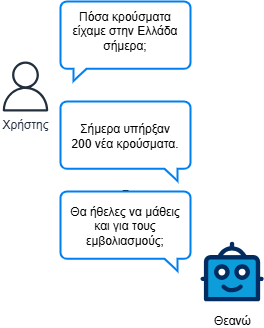
\includegraphics[width=0.4\textwidth]{body_matter/introduction/images/theano_example.png}
    \caption{Παράδειγμα διαλόγου της Θεανώς με χρήστη}
    \label{fig:theano_dialogue}
\end{figure}

Κάνοντας χρήση των παραπάνω ικανοτήτων, η Θεανώ μπορεί να απαντήσει ερωτήσεις σχετικά με τα εμβόλια, την κατάσταση των εμβολιασμών
τόσο στην Ελλάδα όσο και στο εξωτερικό, την κατάσταση των ΜΕΘ, και άλλα παρόμοια θέματα. Επιπλέον, η Θεανώ, στην βασική της έκδοση,
έχει την δυνατότητα να προτείνει τυχαία θέματα για να συνεχίσει την ροή της συζήτηση. Η πρόταση αυτή γίνεται μαζί με την απάντηση του
ερωτήματος που έχει θέσει ο χρήστης. Με αυτό τον τρόπο, η Θεανώ προσπαθεί να ((κρατήσει)) τον χρήστη περισσότερο στην συζήτηση και να τον βοηθήσει
να μάθει περισσότερα πράγματα. Η χρήση αυτής της βασικής μορφής συστάσεων, δείχνει να συνεισφέρει στην μεγαλύτερη διάρκεια των διαλόγων μεταξύ
χρήστη και Θεανώς. Όμως, η συχνή τους χρήση μπορεί να οδηγήσει τον χρήστη να αισθάνεται ότι η Θεανώ δεν τον καταλαβαίνει. Ένα ενδεικτικό παράδειγμα διαλόγου μεταξύ χρήστη
και Θεανώς φαίνεται στο Σχήμα \ref{fig:theano_dialogue}.

Στόχος μας στην εργασία είναι η βελτίωση του συστήματος συστάσεων με στόχο να επιτύχουμε τόσο την μεγαλύτερη διάρκεια των διαλόγων, αλλά ταυτόχρονα
να αυξήσουμε και το αίσθημα των χρηστών ότι η Θεανώ τους καταλαβαίνει και τους συναισθάνεται.

\section{Η συνεισφορά μας}

Σκοπός της εργασίας είναι η δημιουργία ενός συστήματος συστάσεων το οποίο θα διαλειτουργεί με το προϋπάρχον σύστημα της Θεανώς και θα παρέχει διαλογικές
συστάσεις στα θέματα που θα κρατήσουν το ενδιαφέρον του χρήστη για περισσότερους διαλογικούς γύρους.

Για την υλοποίηση αυτού του σκοπού χρησιμοποιήσαμε τεχνικές μηχανικής μάθησης, και πιο συγκεκριμένα, ενισχυτικής μάθησης. Επιλέξαμε να μην χρησιμοποιήσουμε
τεχνικές βαθειάς μηχανικής μάθησης, καθώς το πλήθος των δεδομένων που είχαμε διαθέσιμα δεν μας το επέτρεπε. Επιλέξαμε να χρησιμοποιήσουμε
μια οικογένεια μεθόδων, οι οποίες ονομάζονται \en{bandits}, και ουσιαστικά αποτελούν απλοποίηση του προβλήματος ενισχυτικής μάθησης.

Για την εφαρμογή των μεθόδων \en{bandits} στην εργασία, χρησιμοποιήσαμε το εργαλείο \en{Vowpal Wabbit}, το οποίο προσφέρει έτοιμες πολιτικές \en{bandits},
καθώς και εργαλεία για σύγχρονη εκμάθηση των πολιτικών αυτών. Επιπλέον, για την καλύτερη ροή πληροφορίας μεταξύ του συστήματος συστάσεων και της Θεανώς, τα δύο αυτά συστήματα
διαχωρίστηκαν, και δημιουργήθηκε μια νέα μικρο-υπηρεσία (\en{micro-service}) η οποία είναι υπεύθυνη για τις συστάσεις. Αυτό τελικά σημαίνει ότι η υπηρεσία
και η λειτουργικότητα των συστάσεων είναι μεταφέρσιμη και σε άλλα περιβάλλοντα.

Το σύστημα συστάσεων εκπαιδεύτηκε αρχικά με την χρήση ασύγχρονης εκμάθησης (\en{offline learning}) και μετέπειτα εκπαιδεύεται μέσω της αλληλεπίδρασης του
με τους χρήστες της Θεανώς. Έτσι μπορεί να ακολουθήσει τα ρεύματα και τα ενδιαφέροντα των χρηστών καθώς αυτά αλλάζουν με τον χρόνο.
Τέλος, η υπηρεσία των συστάσεων σχεδιάστηκε με τρόπο που να είναι εύκολα μεταφέρσιμη σε άλλους διαλογικούς πράκτορες σχεδιασμένους με τα εργαλεία του
\en{Rasa}, με μικρές τροποποιήσεις στον περιβάλλοντα κώδικα.

\section{Διάρθρωση της εργασίας}

Στο Κεφάλαιο \ref{chap:rl} παρουσιάζονται οι βασικές γνώσεις Ενισχυτικής Μάθησης. Το κεφάλαιο αυτό παρέχει όλες τις απαραίτητες πληροφορίες για την κατανόηση της
λειτουργίας των τεχνικών \en{bandits}, οι οποίες παρουσιάζονται αναλυτικότερα στο Κεφάλαιο \ref{chap:bandits}, μαζί με τους βασικότερους αλγορίθμους που χρησιμοποιούνται σήμερα.
Έπειτα, στο Κεφάλαιο \ref{chap:dialogue_and_recommendations} παρουσιάζονται συνοπτικά οι βασικές ιδέες γύρω από τα διαλογικά συστήματα και την λειτουργία τους. Στο Κεφάλαιο \ref{chap:ourwork}
παρουσιάζεται αναλυτικά η δική μας εργασία και συνεισφορές. Κλείνοντας, στο Κεφάλαιο \ref{chap:results}, προτείνονται ιδέες για περαιτέρω εξερεύνηση, καθώς και τα σημαντικότερα αποτελέσματα.
